\begin{frame}{Ευθυγράμμιση πανοραμικών σαρώσεων από ευθυγράμμιση εικόνων}


  \begin{figure}
    



\tikzset{every picture/.style={line width=0.75pt}} %set default line width to 0.75pt

\begin{tikzpicture}[x=0.75pt,y=0.75pt,yscale=-1,xscale=1]
%uncomment if require: \path (0,321); %set diagram left start at 0, and has height of 321

%Image [id:dp6846645147891433]
\draw (144.63,99.79) node  {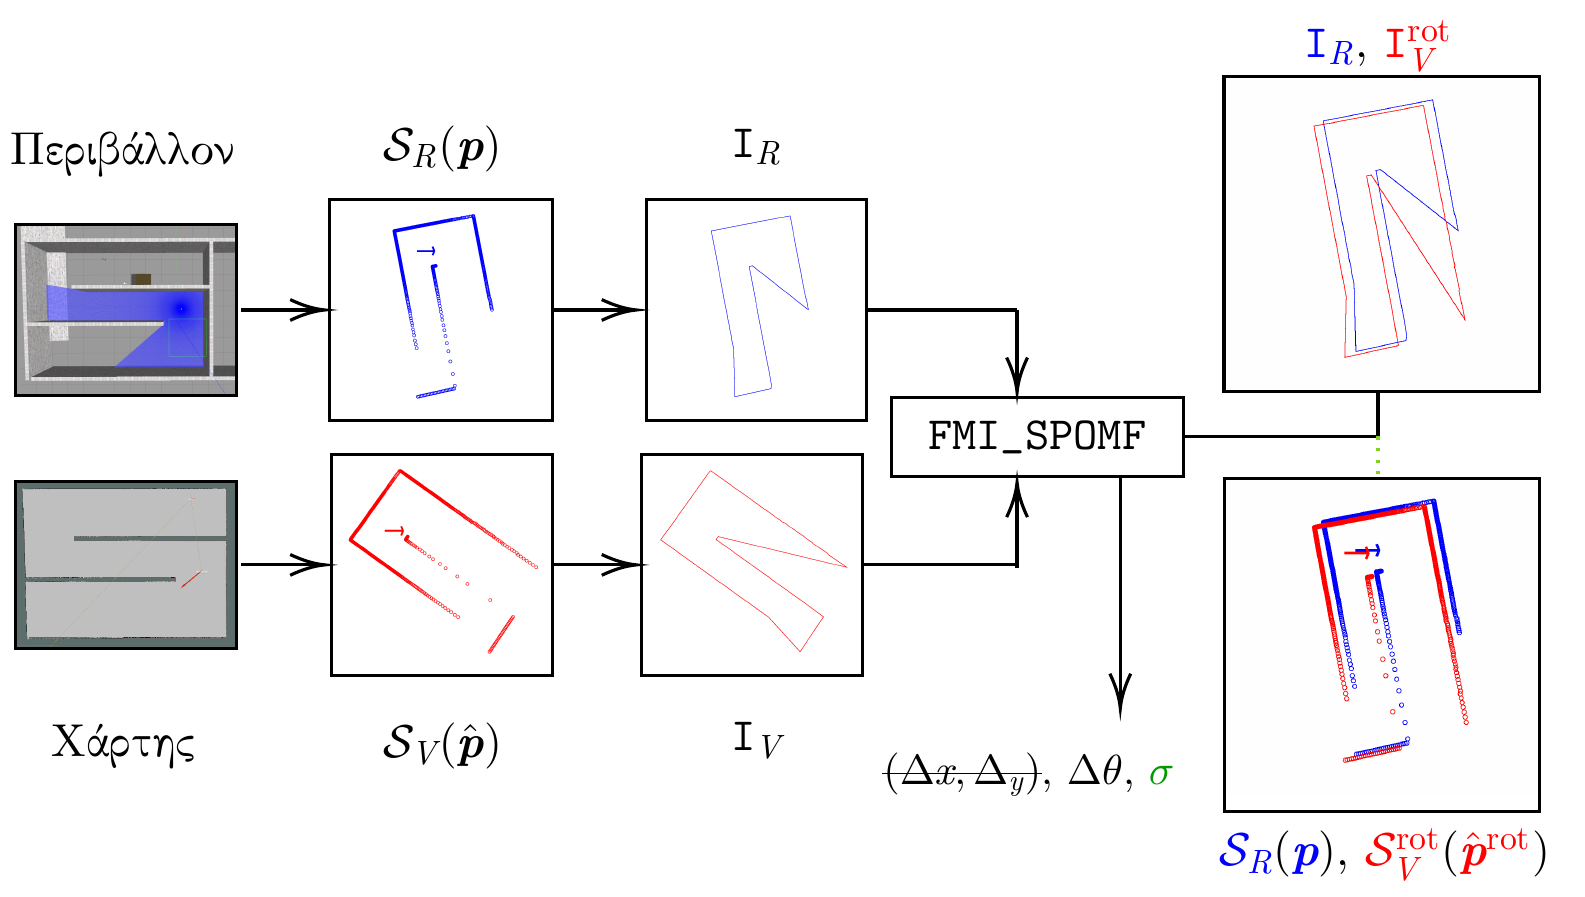
\includegraphics[width=204.19pt,height=114.43pt]{./figures/slides/ch5/scan_to_image/spomf_block.png}};
%Shape: Rectangle [id:dp5629397855877305]
\draw   (8.5,23.5) -- (280.75,23.5) -- (280.75,176.07) -- (8.5,176.07) -- cycle ;
%Shape: Rectangle [id:dp37410715691845486]
\draw  [color={rgb, 255:red, 0; green, 0; blue, 155 }  ,draw opacity=1 ] (63.5,56) -- (104.83,56) -- (104.83,96.5) -- (63.5,96.5) -- cycle ;
%Straight Lines [id:da6833357615020497]
\draw [color={rgb, 255:red, 0; green, 0; blue, 0 }  ,draw opacity=1 ]   (84.17,39) -- (84.17,4) -- (344.17,4.33) -- (344.24,32) ;
\draw [shift={(344.25,34)}, rotate = 269.84] [color={rgb, 255:red, 0; green, 0; blue, 0 }  ,draw opacity=1 ][line width=0.75]    (10.93,-4.9) .. controls (6.95,-2.3) and (3.31,-0.67) .. (0,0) .. controls (3.31,0.67) and (6.95,2.3) .. (10.93,4.9)   ;
%Image [id:dp3924664340729733]
\draw (248,223.75) node  {\animategraphics[width=52.5pt,height=39.38pt,autoplay,loop]{2}{./figures/slides/ch5/scan_to_image/s12_rot_and_trans/sv_}{6}{13}};
%Straight Lines [id:da9897409235946688]
\draw [color={rgb, 255:red, 255; green, 0; blue, 0 }  ,draw opacity=1 ]   (88.25,255) -- (298.75,253.5) -- (298.25,95.5) -- (324.75,95.96) ;
\draw [shift={(326.75,96)}, rotate = 181.01] [color={rgb, 255:red, 255; green, 0; blue, 0 }  ,draw opacity=1 ][line width=0.75]    (10.93,-3.29) .. controls (6.95,-1.4) and (3.31,-0.3) .. (0,0) .. controls (3.31,0.3) and (6.95,1.4) .. (10.93,3.29)   ;
%Straight Lines [id:da5830453979317929]
\draw    (344.25,76.5) -- (344.25,60) ;
\draw [shift={(344.25,78.5)}, rotate = 270] [color={rgb, 255:red, 0; green, 0; blue, 0 }  ][line width=0.75]    (10.93,-4.9) .. controls (6.95,-2.3) and (3.31,-0.67) .. (0,0) .. controls (3.31,0.67) and (6.95,2.3) .. (10.93,4.9)   ;
%Straight Lines [id:da5230753835364603]
\draw    (345.25,131.5) -- (345.25,116) ;
\draw [shift={(345.25,114)}, rotate = 90] [color={rgb, 255:red, 0; green, 0; blue, 0 }  ][line width=0.75]    (10.93,-4.9) .. controls (6.95,-2.3) and (3.31,-0.67) .. (0,0) .. controls (3.31,0.67) and (6.95,2.3) .. (10.93,4.9)   ;
%Straight Lines [id:da416994847189329]
\draw [color={rgb, 255:red, 0; green, 0; blue, 0 }  ,draw opacity=1 ]   (344.75,159.5) -- (344.75,222.5) -- (282.75,222.5) ;
\draw [shift={(344.75,157.5)}, rotate = 90] [color={rgb, 255:red, 0; green, 0; blue, 0 }  ,draw opacity=1 ][line width=0.75]    (10.93,-4.9) .. controls (6.95,-2.3) and (3.31,-0.67) .. (0,0) .. controls (3.31,0.67) and (6.95,2.3) .. (10.93,4.9)   ;
%Image [id:dp41388351298947]
\draw (479.88,96.16) node  {\animategraphics[width=115.31pt,height=86.48pt,autoplay,loop]{2}{./figures/slides/ch5/scan_to_image/s12_rot_and_trans/both_}{6}{13}};
%Straight Lines [id:da5700236263242655]
\draw [color={rgb, 255:red, 255; green, 0; blue, 0 }  ,draw opacity=1 ]   (358.75,96) -- (386.75,96) ;
%Shape: Rectangle [id:dp5216838625830877]
\draw   (213,197.5) -- (283,197.5) -- (283,250) -- (213,250) -- cycle ;
%Straight Lines [id:da52359587642321]
\draw [color={rgb, 255:red, 255; green, 0; blue, 0 }  ,draw opacity=1 ]   (386.25,95.5) -- (386.75,257) -- (69.75,257) ;
%Straight Lines [id:da439821987039549]
\draw [color={rgb, 255:red, 0; green, 0; blue, 0 }  ,draw opacity=1 ]   (189.25,223.5) -- (207.75,223.95) ;
\draw [shift={(209.75,224)}, rotate = 181.4] [color={rgb, 255:red, 0; green, 0; blue, 0 }  ,draw opacity=1 ][line width=0.75]    (10.93,-3.29) .. controls (6.95,-1.4) and (3.31,-0.3) .. (0,0) .. controls (3.31,0.3) and (6.95,1.4) .. (10.93,3.29)   ;
%Straight Lines [id:da29976143449805104]
\draw [color={rgb, 255:red, 255; green, 0; blue, 0 }  ,draw opacity=1 ]   (69.75,257) -- (70.19,242) ;
\draw [shift={(70.25,240)}, rotate = 91.68] [color={rgb, 255:red, 255; green, 0; blue, 0 }  ,draw opacity=1 ][line width=0.75]    (10.93,-4.9) .. controls (6.95,-2.3) and (3.31,-0.67) .. (0,0) .. controls (3.31,0.67) and (6.95,2.3) .. (10.93,4.9)   ;
%Straight Lines [id:da9524081777716664]
\draw [color={rgb, 255:red, 0; green, 0; blue, 0 }  ,draw opacity=1 ]   (28.17,190.67) -- (149,190) -- (149,207) ;
\draw [shift={(149,209)}, rotate = 270] [color={rgb, 255:red, 0; green, 0; blue, 0 }  ,draw opacity=1 ][line width=0.75]    (10.93,-3.29) .. controls (6.95,-1.4) and (3.31,-0.3) .. (0,0) .. controls (3.31,0.3) and (6.95,1.4) .. (10.93,3.29)   ;
%Straight Lines [id:da930420365372618]
\draw [color={rgb, 255:red, 0; green, 0; blue, 0 }  ,draw opacity=1 ]   (264.75,178.5) -- (264.25,185) -- (70.25,185) -- (70.25,208) ;
\draw [shift={(70.25,210)}, rotate = 270] [color={rgb, 255:red, 0; green, 0; blue, 0 }  ,draw opacity=1 ][line width=0.75]    (10.93,-3.29) .. controls (6.95,-1.4) and (3.31,-0.3) .. (0,0) .. controls (3.31,0.3) and (6.95,1.4) .. (10.93,3.29)   ;
%Shape: Rectangle [id:dp2812144239172756]
\draw  [color={rgb, 255:red, 255; green, 0; blue, 0 }  ,draw opacity=1 ] (10,104) -- (50.17,104) -- (50.17,135.33) -- (10,135.33) -- cycle ;
%Straight Lines [id:da41545421882941236]
\draw [color={rgb, 255:red, 0; green, 0; blue, 0 }  ,draw opacity=1 ]   (28.83,157.67) -- (28.17,190.67) ;
%Shape: Square [id:dp9207499552838876]
\draw  [color={rgb, 255:red, 0; green, 0; blue, 0 }  ,draw opacity=1 ] (256,159.67) -- (274.83,159.67) -- (274.83,178.5) -- (256,178.5) -- cycle ;
%Shape: Circle [id:dp5995835539431238]
\draw   (330.25,96) .. controls (330.25,87.99) and (336.74,81.5) .. (344.75,81.5) .. controls (352.76,81.5) and (359.25,87.99) .. (359.25,96) .. controls (359.25,104.01) and (352.76,110.5) .. (344.75,110.5) .. controls (336.74,110.5) and (330.25,104.01) .. (330.25,96) -- cycle ;
%Shape: Rectangle [id:dp8131628175009749]
\draw  [line width=2.25]  (402.25,36) -- (565.25,36) -- (565.25,155.5) -- (402.25,155.5) -- cycle ;
%Straight Lines [id:da24561475378348807]
\draw  [dash pattern={on 0.75pt off 0.75pt}]  (386.25,95.5) .. controls (388.02,93.94) and (389.68,94.04) .. (391.24,95.81) .. controls (392.8,97.58) and (394.46,97.68) .. (396.23,96.12) .. controls (398,94.57) and (399.66,94.67) .. (401.22,96.44) -- (402.25,96.5) -- (402.25,96.5) ;
%Straight Lines [id:da23644770211611]
\draw [color={rgb, 255:red, 255; green, 0; blue, 0 }  ,draw opacity=1 ]   (79.75,224.5) -- (107.75,224.5) ;
\draw [shift={(109.75,224.5)}, rotate = 180] [color={rgb, 255:red, 255; green, 0; blue, 0 }  ,draw opacity=1 ][line width=0.75]    (10.93,-3.29) .. controls (6.95,-1.4) and (3.31,-0.3) .. (0,0) .. controls (3.31,0.3) and (6.95,1.4) .. (10.93,3.29)   ;
%Straight Lines [id:da15890574239196265]
\draw [color={rgb, 255:red, 255; green, 0; blue, 0 }  ,draw opacity=1 ]   (88.25,255) -- (88.25,224.5) ;

% Text Node
\draw (138,12) node [anchor=north west][inner sep=0.75pt]  [font=\tiny] [align=left] {Υποσύστημα εκτίμησης προσανατολισμού};
% Text Node
\draw    (309.19,37) -- (381.19,37) -- (381.19,58) -- (309.19,58) -- cycle  ;
\draw (345.19,47.5) node  [font=\footnotesize] [align=left] {Βαρύκεντρο};
% Text Node
\draw    (309.19,134) -- (381.19,134) -- (381.19,155) -- (309.19,155) -- cycle  ;
\draw (345.19,144.5) node  [font=\footnotesize] [align=left] {Βαρύκεντρο};
% Text Node
\draw (356.5,61.5) node [anchor=north west][inner sep=0.75pt]   [align=left] {+};
% Text Node
\draw (356.5,112.5) node [anchor=north west][inner sep=0.75pt]   [align=left] {\mbox{-}};
% Text Node
\draw    (112.61,211.5) -- (189.61,211.5) -- (189.61,236.5) -- (112.61,236.5) -- cycle  ;
\draw (151.11,226) node   [align=left] {\texttt{scan\_map}};
% Text Node
\draw    (62.5,212.5) -- (79.5,212.5) -- (79.5,237.5) -- (62.5,237.5) -- cycle  ;
\draw (65,217) node [anchor=north west][inner sep=0.75pt]   [align=left] {$\hat{\bm{p}}$};


\end{tikzpicture}

  \end{figure}

\note{\footnotesize
Για την εκτίμηση της μετατόπισης ανάμεσα στις δύο σαρώσεις χρησιμοποιούμε μία
μέθοδο η οποία εφαρμόζεται μετά την περιστροφή της δεύτερης σάρωσης ως προς την
πρώτη. Η μέθοδος αυτή υπολογίζει το βαρύκεντρο των δύο σαρώσεων στο
καρτεσιανό επίπεδο και μεταφέρει τη δεύτερη σάρωση ώστε να συμπέσει με την
πρώτη με βάση τη διαφορά των κεντροειδών τους. Για τον υπολογισμό της
μετατόπισης δεν χρησιμοποιούνται πουθενά αντιστοιχίσεις, διότι τα κεντροειδή
υπολογίζονται προφανώς το ένα ανεξάρτητα από το άλλο.
}

\end{frame}
